%\chapterauthor{Author Name}{Author Affiliation}
%\chapterauthor{Second Author}{Second Author Affiliation}
\chapter{Process Management} \label{ch:pm}

A process refers to an instance of a computer program that is running in the system. Managing processes is one of the essential tasks of an OS. In a Windows system, the user can use the task manager, a graphical tool, to check and manage all the running processes. In a Linux system, the user can manage process in the prompt console using bash commands.

\section{General Introduction to Process}

A \mync{process}, also known as \mync{task}, represents an instance of a program or an application that is being executed on the machine. The OS manages the applications and their corresponding required resources by managing the processes.
\subsection{Process}

To improve the efficiency of the system, especially \myabb{Central Processing Unit}{CPU}, the OS allows multiple processes to share the computational capability and memory of the system, each thinking that it is exclusively using the all machine resources, as shown in Fig. \ref{ch:pm:fig:processflow}.

\begin{figure}[!htb]
	\centering
	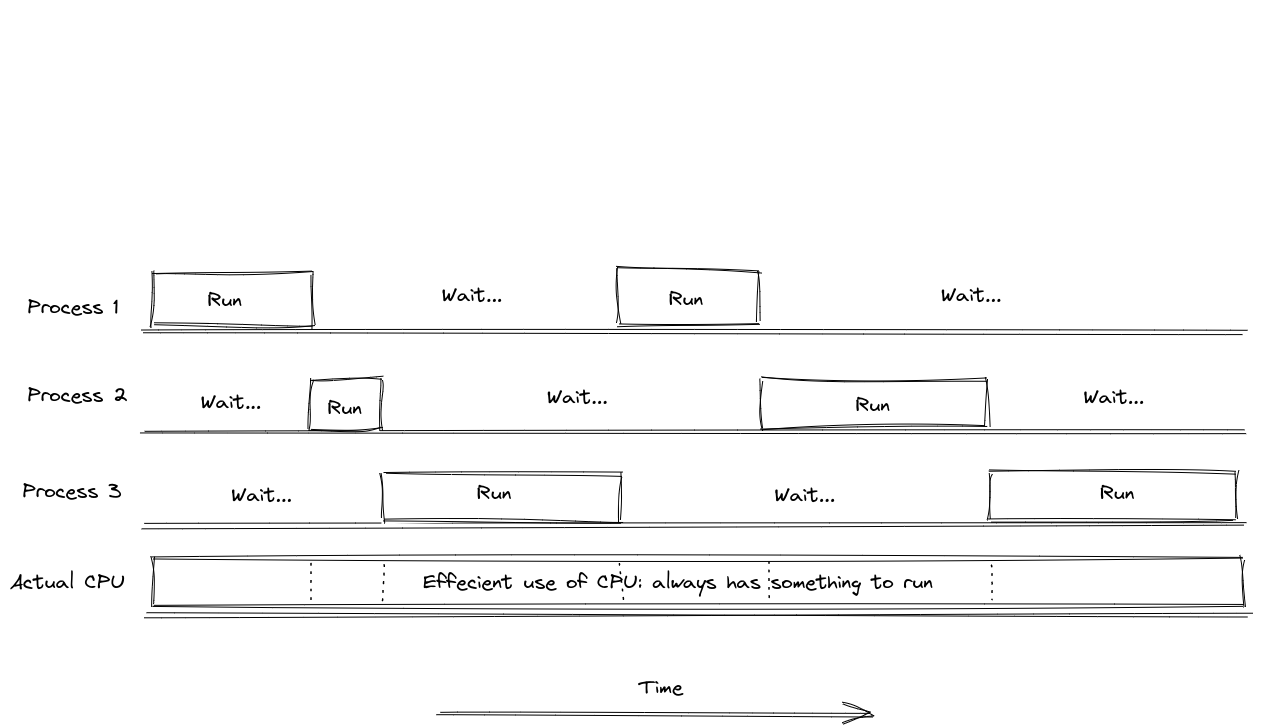
\includegraphics[width=350pt]{chapters/part-1/figures/processflow.png}
	\caption{A demonstration of running multiple processes on a single-core CPU.} \label{ch:pm:fig:processflow}
\end{figure}

The status and context of a process are stored in its \mync{Process Control Block}[PCB]. The PCB is a special data structure used to describe the metadata and the dynamic of a process. The OS manages the PCBs and control the processes accordingly. Some of the attributes of a PCB are summarized in Table \ref{ch:pm:tab:pcbcontent}.

\begin{table}[!htb]
	\centering \caption{Some attributes of a PCB.}\label{ch:pm:tab:pcbcontent}
	\begin{tabularx}{\textwidth}{lX}
		\hline
		Name & Description \\ \hline
		Process ID & The unique ID of the process.  \\
		State & The state of the process, for example, running, suspended, terminated.  \\
		Priority & Priority level in comparison with other processes. \\
		Program Counter & A pointer to the next line of program to be executed. \\
		Memory regions & A pointer to the RAM where the code and data of the process is stored. \\
		Accounting Information & Time limits, clock time used, etc. \\ \hline
	\end{tabularx}
\end{table}

Fig.~\ref{ch:pm:fig:processstatetransfer} shows the possible states that a process might be at. Note the differences between ``blocked'' and ``suspended''. ``Block'' indicates that the process is waiting for other inputs to carry out the remaining part of the program, and ``suspended'' indicates that the process is put on hold for some reasons. When a process is offloaded from the CPU, its context is moved from the CPU registers to the PCB of the progress.

\begin{figure}[!htb]
	\centering
	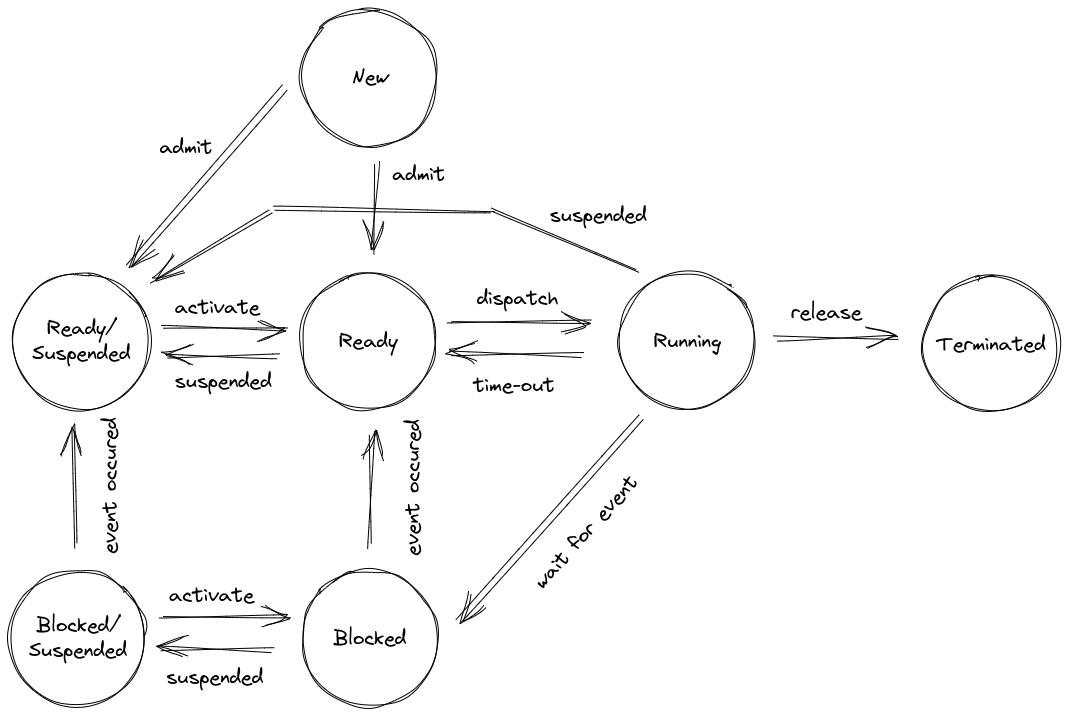
\includegraphics[width=350pt]{chapters/part-1/figures/processstatetransfer.png}
	\caption{Fundamental states of a process and their transferring.} \label{ch:pm:fig:processstatetransfer}
\end{figure}

There are different types of processes. For example, based on the source of the processes, there are OS triggered processes and user triggered processes, the first of which usually have a higher priority. Based on the running environment, there are front-ground processes and background processes. Based on the resources used, there are CPU processes and I/O processes.

A process usually has a relatively isolated environment, and it does not share memory storage with other processes. Special inter process communication mechanism, which is often referred as ``pipe'', is required for processes to talk to each other. Inter-process communication requires OS level controls.

\subsection{Thread}

A \mync{thread} is like a work dispatch inside a process. There can be multiple threads in a process, as shown in Fig \ref{ch:pm:fig:threadinprocess}. Each thread has its own CPU register values and stack, but they share the same program, memory and file storage addresses.
\begin{figure}[!htb]
	\centering
	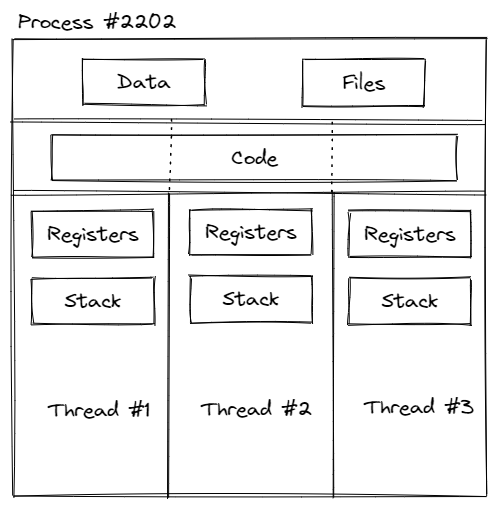
\includegraphics[width=200pt]{chapters/part-1/figures/threadinprocess.png}
	\caption{A demonstration of multiple threads in a process.} \label{ch:pm:fig:threadinprocess}
\end{figure}

Threads differ from processes in the following aspects:
\begin{itemize}
  \item A thread is lighter than a process, occupying less resources to create.
  \item Sharing memories and resources among threads in a process is easier than sharing among processes, because they naturally share address space.
  \item It is easier to enable parallel computation for the threads in the process when it is running on a multi-core CPU.
\end{itemize}

Notice that for many OS, including Linux, the kernel can provide thread level services.

\section{Process Management in Linux}

Basic process management commands including monitoring and terminating a process are given. Switching a process between foreground and background is also introduced.

\subsection{Monitor}

Two commands, \verb|ps| and \verb|top|, are widely used in monitoring the running process in the OS. They can be used stand-alone, without additional arguments as follows.
\begin{lstlisting}
$ ps [options]
\end{lstlisting}
or
\begin{lstlisting}
$ top
\end{lstlisting}

The major difference between these two commands is that \verb|ps| provides a snapshot (in a text format) of a list of processes, each with its name, \myabb{Process ID}{PID} and owner, etc., while \verb|top| provides a dynamic and frequently refreshing display of the running processes as well as their associated resources usage. Figs \ref{ch:pm:fig:pscommand} and \ref{ch:pm:fig:topcommand} give a quick demo of how the execution of the two commands look like.

\begin{figure}[!htb]
	\centering
	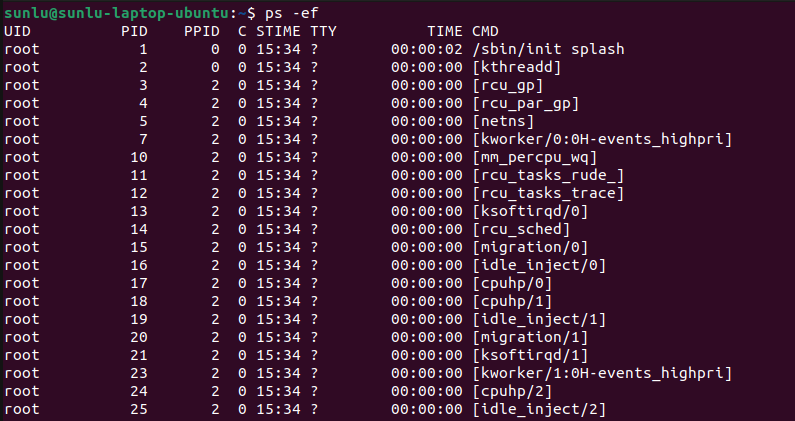
\includegraphics[width=300pt]{chapters/part-1/figures/pscommand.png}
	\caption{Execution of \texttt{ps -ef} command.} \label{ch:pm:fig:pscommand}
\end{figure}

\begin{figure}[!htb]
	\centering
	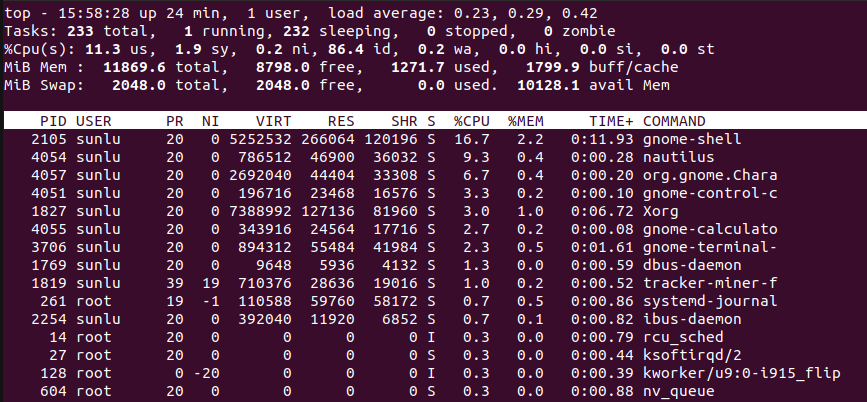
\includegraphics[width=300pt]{chapters/part-1/figures/topcommand.png}
	\caption{Execution of \texttt{top} command.} \label{ch:pm:fig:topcommand}
\end{figure}

Notice that \verb|top| is a running application where the user can keep interacting with to filter for particular processes, while \verb|ps| is more of a one-time command and its output can be saved into a text file for further processing.

Some commonly used options for \verb|ps| are summarized below.
\begin{itemize}
	\item \verb|-e|: list all processes
	\item \verb|-f|: list details of the processes
	\item \verb|-C <command name>| filter by command
	\item \verb|-u <username>| filter by user
\end{itemize}

\subsection{Termination}

To kill a process, use the \verb|kill| command as follows.
\begin{lstlisting}
$ kill <option> <process ID>
\end{lstlisting}

The \verb|kill| command offers different options to kill a process. Use \verb|kill -l| to list down the options as given below (and many more).
\begin{lstlisting}
1) SIGHUP    2) SIGINT    3) SIGQUIT   4) SIGILL
5) SIGTRAP   6) SIGABRT   7) SIGBUS    8) SIGFPE
9) SIGKILL  10) SIGUSR1  11) SIGSEGV  12) SIGUSR2
13) SIGPIPE 14) SIGALRM	 15) SIGTERM  16) SIGSTKFLT
17) SIGCHLD 18) SIGCONT	 19) SIGSTOP  20) SIGTSTP
...
\end{lstlisting}

Commonly used \verb|kill| options are \verb|kill -9| (SIGKILL) and \verb|kill -15| (SIGTERM) followed by the PID. It is mostly recommended to use \verb|kill -15| over \verb|kill -9|, as it allows the process to clean up and terminate properly. Most well designed software defines the protocol to terminate the process in a safe way. This is also the default termination option. Command \verb|kill -9|, on the other hand, force the OS to terminate the process immediately. It is used mostly when the process is not responding and cannot be terminated using \verb|kill -15|.

Another command \verb|killall| runs similarly as \verb|kill|, except that it kills signals based on the command, not the process ID. As a result, it is possible to use it to kill multiple signals with the same command at a time. Use it with cautions.

Notice that in Linux the process is arranged in a tree structure; killing a parent process will automatically terminate its children processes, and killing a child process may result in its parent process to restart a new child process.

\subsection{Switching between Foreground and Background}

To start a command as a background process, use \verb|&| in the end of the command as follows
\begin{lstlisting}
$ <command> &
\end{lstlisting}
This is useful if a command is time consuming and it does not need additional user interaction while running.

To check commands running in the background, use
\begin{lstlisting}
$ jobs
[1] <status> <command>
[2] <status> <command>
[3]+ <status> <command>
[4]- <status> <command>
...
\end{lstlisting}
A plus sign ``\verb|+|'' indicates that the command was the most recent one placed in the background, and the minus sign ``\verb|-|'', the second most recent one. To bring a background command to the foreground, use
\begin{lstlisting}
$ fg %<job number>
\end{lstlisting}
where \verb|<job number>| is the index given in \verb|jobs| outputs. If no job number is given, the most recent job will be brought to the foreground.

\subsection{Process Priority Manipulation}

The \mync{priority}[PR] of a process is given by an integer between $-100$ and $39$, the smaller the more prioritized. This value can be viewed using \verb|top|, as shown in Fig. \ref{ch:pm:fig:topcommand} under column ``PR''. The process with priority $-100$ is displayed as \verb|rt|, indicating the highest priority.

The entire priority range from $-100$ to $39$ is divided into two portions. The priority between $-100$ and $-1$ is known as ``real-time'', and between $0$ and $39$, ``normal''. In practice, real-time processes are mainly managed by the root user and are not accessible to regular users. A regular user's process typically falls within the normal priority range of $0$ to $39$. 

A ``\mync{NICE value}'' is assigned to the priorities. The priority $0$ corresponds with NICE value of $-20$, and $39$ with $19$. The user can adjust the NICE value of his process and hence change its priority. This is demonstrated by Fig. \ref{ch:pm:fig:priority}.

\begin{figure}[htbp]
	\centering
	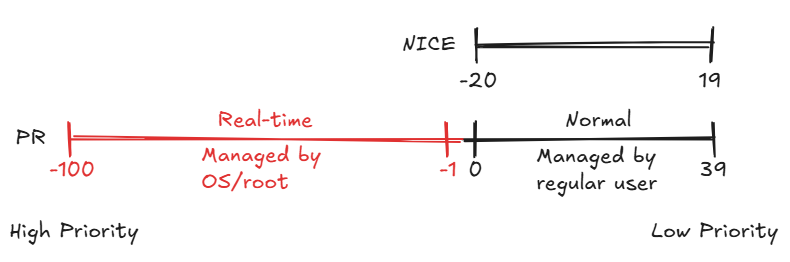
\includegraphics[width=300pt]{chapters/part-1/figures/priority.png}
	\caption{Priority levels in Linux.} \label{ch:pm:fig:priority}
\end{figure}

For normal processes, their NICE values can be viewed using \verb|top| as shown in Fig. \ref{ch:pm:fig:topcommand} under column ``NI''. Real-time processes do not use NICE value, hence NI are displayed as $0$ for these processes.

A properly designed OS should have built-in algorithms to manage process priorities and scheduling. However, tools like \verb|nice| and \verb|renice| are provided to give users and administrators the ability to manipulate these priorities in specific situations. Examples are given below.

To run a command with a specified NICE value, use
\begin{lstlisting}
$ nice -n <increment> <command>
\end{lstlisting}
and \verb|<increment>| will be the NICE value of the command.

To change the NICE value of an existing process, use
\begin{lstlisting}
$ renice -n <increment> -p <prosess id>
\end{lstlisting}
where \verb|<increment>|, being either positive or negative, will be added to the current NICE value of the process with the specified process ID.

It is also possible to manage the priorities not by individual process ID, but by a group of processes. This is useful when a group of processes belongs to a similar service or to a group of users, and we want to change the priority of the service or users all together.


